\title{DEVELOPMENT and Output}
\begin{center}
    \textbf{Chapter 06}\\
    \section{\large \textbf{DEVELOPMENT INPUT AND OUTPUT}}
\end{center}
\vspace{2.5mm}
\subsection{Introduction}
The introduction of the Employee Management System (EMS) project report provides an
overview of the development inputs and outputs crucial for the successful implementation
of the system. Development inputs encompass the resources, tools, and expertise required
throughout the project lifecycle. This includes the technical skills of software developers,
database administrators, and domain experts, as well as hardware and software
infrastructure needed for testing and deployment. Additionally, user feedback and
requirements gathered from stakeholders contribute to shaping the EMS's functionalities.
On the other hand, development outputs refer to the tangible results produced during the
project, such as the EMS's fully functional modules, the integrated database, and the user
interface. The report outlines the significance of these inputs and outputs in achieving the
project's objectives, ensuring an efficient, user-friendly, and scalable EMS that optimizes
employee management processes. Throughout the subsequent sections, this project report
will delve into the specifics of development inputs and outputs, showcasing their pivotal
role in creating a comprehensive and robust Employee Management System.
\newpage
\subsection{Login Page}
The login page in the Employee Management System (EMS) project report is a crucial
component of the system's user interface. It serves as the entry point for authorized users, such
as employees and HR administrators, to access the system and perform various tasks.
\begin{figure}[h]
    \centering
    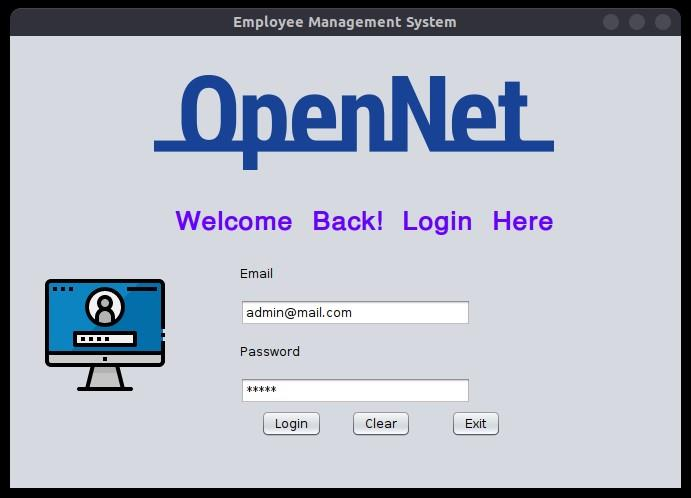
\includegraphics[height=7cm]{img/appsimg/login.png}
    \caption{Login Page}
    \label{fig:login}
\end{figure}
\subsection{Home Page}
The home page will have a header section with a logo, navigation menu, search bar and possibly
some promotional banners or sliders that display current deals or promotions.
\begin{figure}[h]
    \centering
    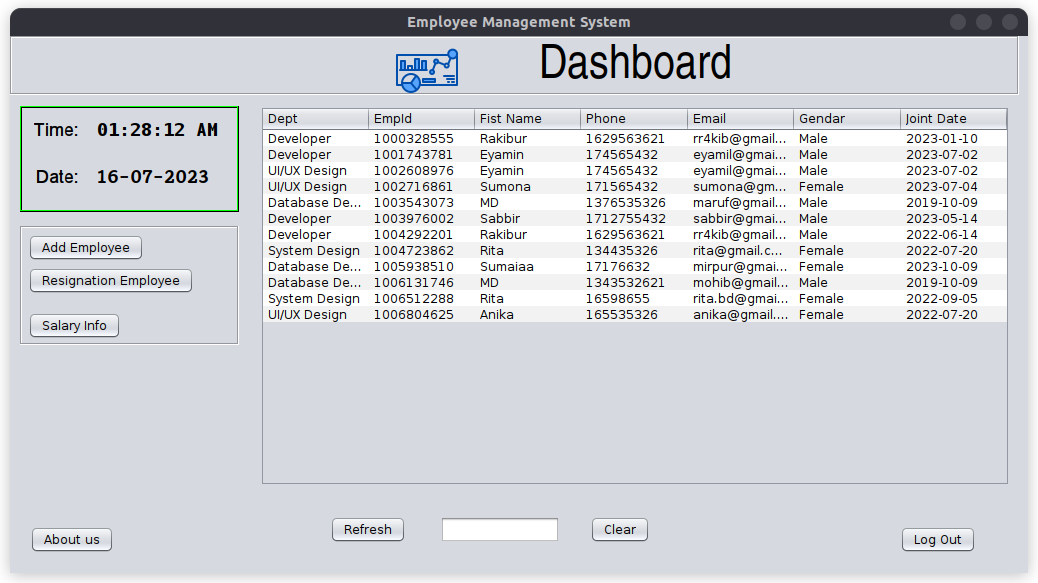
\includegraphics[height=7cm]{img/appsimg/home.png}
    \caption{Home Page or Dashboard}
    \label{fig:hoomepage}
\end{figure}
\subsection{Resignation Employee Page}
The Resignation Employee page in the Employee Management System (EMS) project report is a
component that allows employees to submit their resignation requests through the system. This
page provides a user-friendly interface for employees to initiate the resignation process and
communicates their intention to leave the organization to the HR department.
\begin{figure}[h]
    \centering
    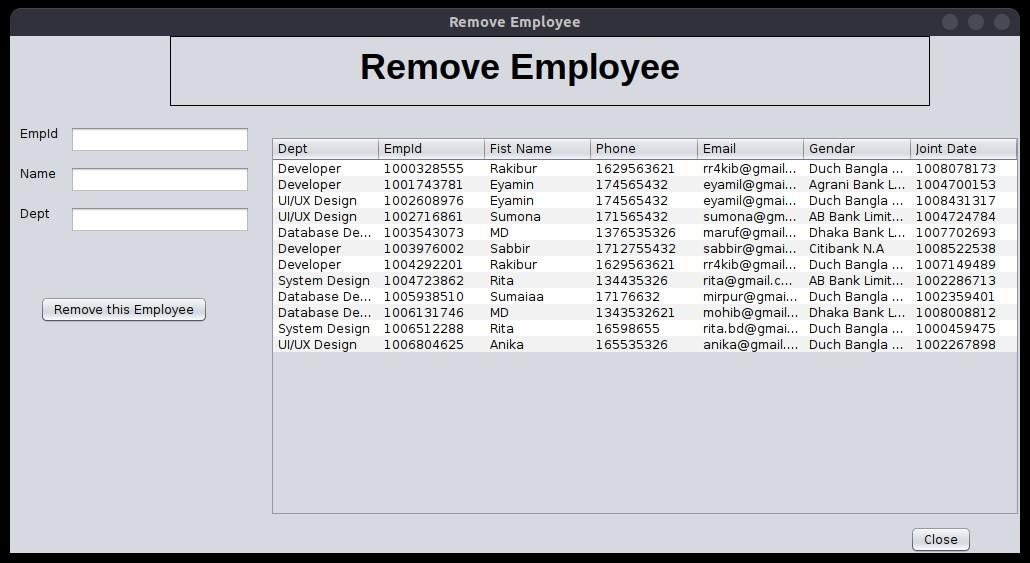
\includegraphics[height=8cm]{img/appsimg/remvoe.png}
    \caption{Resignation Page}
    \label{fig:resig}
\end{figure}
\newpage
\subsection{Add New Employee Page}
The "Add New Employee" page in the Employee Management System (EMS) project report is a
fundamental component that enables HR administrators or authorized personnel to add new
employees to the system. This page provides a user-friendly interface to input and store essential
details of newly hired staff members, facilitating efficient on boarding processes.
\begin{figure}[h]
    \centering
    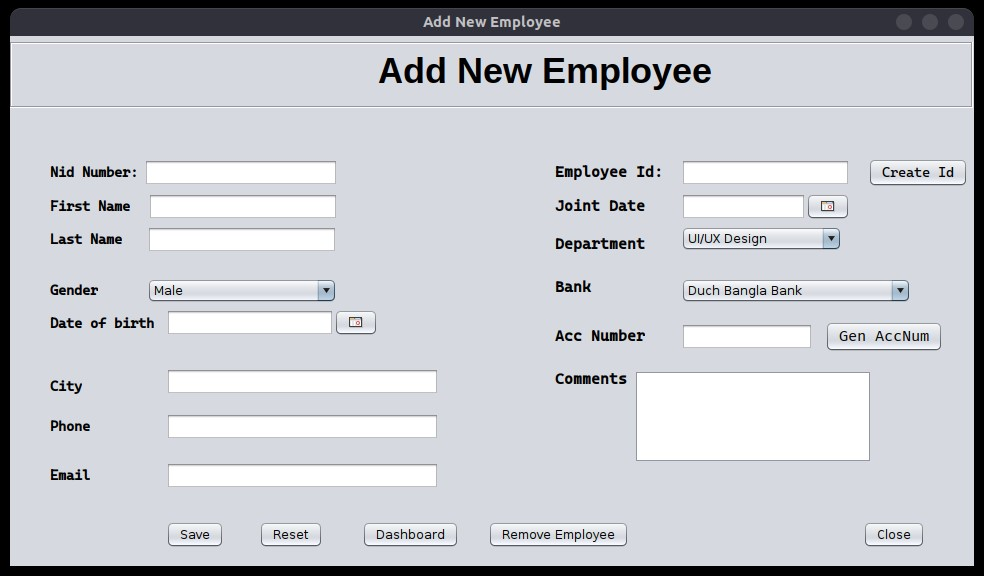
\includegraphics[height=8cm]{img/appsimg/addnwe.png}
    \caption{Add New Employee Page}
    \label{fig:addnewempl}
\end{figure}
\subsection{Salary Page}
The "Salary Page" in the Employee Management System (EMS) project report is a vital component
that enables HR administrators to manage and process employee salaries and related financial
information. This page provides a centralized interface to handle payroll-related tasks efficiently
and accurately.
\begin{figure}[h]
    \centering
    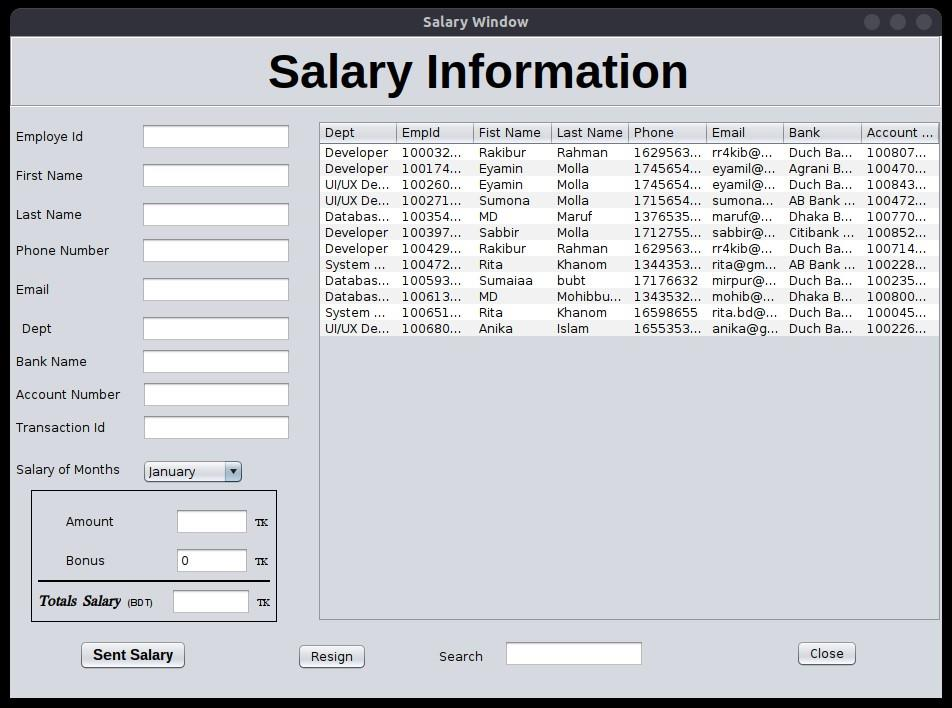
\includegraphics[height=8cm]{img/appsimg/slara.png}
    \caption{Salary Page}
    \label{fig:salary}
\end{figure}
\subsection{About page}
The "About Page" in the Employee Management System (EMS) project report is a section
dedicated to providing essential information about the system and its development. It serves as
a documentation component that offers readers a clear understanding of the project's purpose,
objectives, and key features.
\begin{figure}[h]
    \centering
    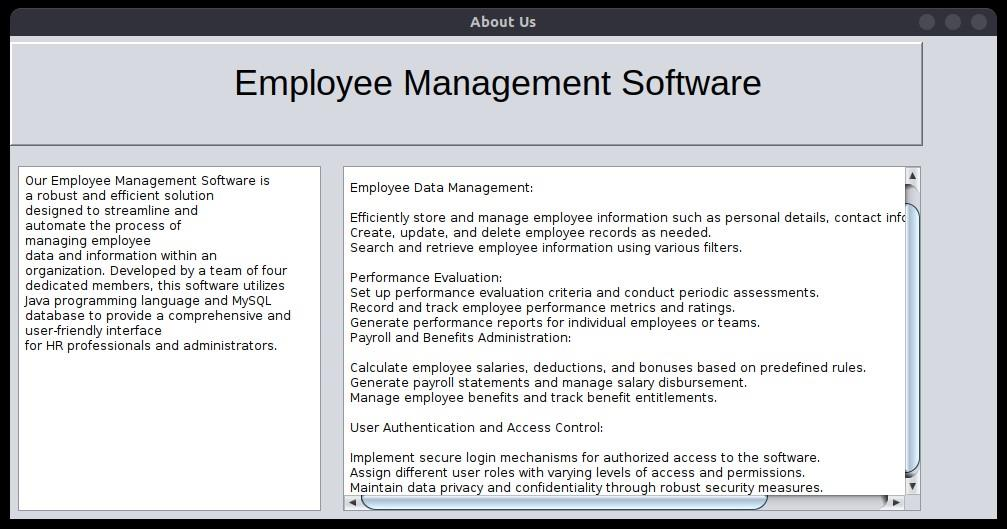
\includegraphics[height=8cm]{img/appsimg/about.png}
    \caption{About Page}
    \label{fig:about}
\end{figure}